\graphicspath{{figures/chapter1/}}

\chapter{Introduction}\label{ch:introduction}
\label{introduction}

\vfill

\newthought{This chapter is based on:}

\noindent 

\begin{itemize}
  \item De Gaetani, C. I., Ioli, F., \& Pinto, L. (2021). Aerial and UAV Images for
Photogrammetric Analysis of Belvedere Glacier Evolution in the Period 1977–2019. Remote
Sensing, 13(18), 3787. \url{https://doi.org/10.3390/rs13183787}
\item Ioli, F., Bianchi, A., Cina, A., De Michele, C., Maschio, P., Passoni, D., \&
Pinto, L. (2021). Mid-Term Monitoring of Glacier’s Variations with UAVs: The Example of the Belvedere Glacier. Remote Sensing, 14(1), 28.
\url{https://doi.org/10.3390/rs14010028}
  \item Ioli, F., Dematteis, N., Giordan, D., Nex, F., Pinto, L. (2024). Deep Learning Low-cost Photogrammetry for 4D Short-term Glacier Dynamics Monitoring. \textit{PFG}. 
  \\\url{https://doi.org/10.1007/s41064-023-00272-w}
\end{itemize}

\newpage

\section{Motivation and relevance}

Glaciers all over the world are experiencing profound transformations due to the ongoing climate crisis~\citep{Oerlemans2005} and their sensitivity to temperature fluctuations renders them powerful indicators of global climate change~\citep{Barry2016}.

Alpine glaciers, situated in temperate zones, are particularly susceptible to rising temperatures. The accelerated rate of glacial retreat underscores the necessity for comprehensive monitoring programs~\citep{Zemp2006,Sommer2020}. 
Therefore, they are often considered as a proxy for climate change evaluation.
Projections point out that the European Alps may lose more than 60\% of ice volume by the end of the century under the RCP2.6 scenario, whereas a larger amount of ice loss is expected under worse scenarios~\citep{Zekollari2019}.

However, mountain glaciers are a critical component of the local economy regarding freshwater supply, hydroelectric production, and tourist activities.
In particular, glaciers serve as critical as crucial freshwater reservoirs and their undergoing transformation is likely to have severe consequences for the future water availability~\citep{Barnett2005, hock2005}. 

Additionally, glacier melting and retreat are triggering several glaciological processes, e.g., ice break-off, glacier outburst, snow/ice avalanches, and gravitational slope stability processes, such as rockfalls and collapses, and debris flow, which can threaten the population, urban areas or infrastructure of the nearby areas~\citep{Kaab2004, Deline2015, Giordan2020}.
In the European Alps, the number of mass movements and hazardous events in the high-elevations environments has experienced an increase in the past decade due to climate change~\citep{chiarle2023, Nigrelli2024}.

A relevant and tragic example was the collapse of a section of the Marmolada Glacier (Dolomites, Italy), which occurred on 3 July 2022 at 13:43:20 CEST. 
The collapse caused an ice avalanche that killed 11 mountaineers trying to reach the Marmolada summit and injured 7~\citep{Olivieri2023, Bondesan2023}.
The collapse occurred on the northern slope of the glacier at an elevation of \SI{3213}{\masl} and involved a volume of \SI{\sim 96000}{\cubic\meter}~\citep{Olivieri2023}.
The detachment was caused by a failure along a median crevasse, partially filled by meltwater due to highly anomalous temperatures, that reached \SI{10.7}{\degree\celsius} at the time of the event.
The sudden glacier collapse was probably induced by a combination of hydraulic jacking and pressure within a thin layer of basal till~\citep{Bondesan2023}.

Just one year after the Marmolada collapse, another relevant event slope instability event was registered in the Austrian state of Tyrol, close to the Italian border. 
On 11 June 2023, a big portion of the summit of Fluchthorn, a nearly \SI{3400}{\masl} has collapsed sending more than \SI{100000}{\cubic\meter} of rock crashing into the valley below and triggering mudslides\footnote{\mbox{\url{https://edition.cnn.com/2023/06/14/europe/austrian-mountain-fluchthorn-rockslide-climate-intl/index.html}}}.
This event was likely related to the thawing permafrost due to the high temperatures of that period\footnote{\url{https://blogs.agu.org/landslideblog/2023/06/12/fluchthorn-1/}}.

In this context, long-term monitoring of glaciers and related glaciological processes assumes increasing significance.
To achieve a thorough understanding of these complex systems, systematic observations are indispensable~\citep{Kaab2005}.
A particular focus is usually placed on monitoring surface kinematics, as these can potentially offer early warning signs of impending instability or collapse events~\citep{Faillettaz2015}.

However, monitoring glaciers in remote areas and inaccessible terrains often presents logistical and safety challenges.
A practical approach is the adoption of remote sensing apparatuses that allow observing glacial processes with minimal risk for scientists and technicians. 


Remote sensing technologies offer a compelling solution, enabling scientists to study glacial processes with greater efficiency and reduced risk to field personnel.

In recent years, the free availability of data acquired from satellite platforms has largely improved the possibility to observe wide areas from remote with relatively high spatiotemporal resolution. Nevertheless, satellite surveys suffer complex geometries and the revisit time might be not adequate to measure fast processes. Therefore, the use of close-range remote sensing systems is often the most effective solution for glacier monitoring [6].

% Mountain glaciers are a crucial element for the local economy in terms of freshwater supply, hydroelectric production, and tourist activities [1]. Glacier surface mass balance, elevation change, and terminus retreat are often quantitatively surveyed to evaluate their current state and recent evolution [2]. However, such monitoring activities are usually conducted periodically (e.g., with seasonal or annual revisit time) due to the investigated processes’ relatively slow dynamics. 

\cite{Paul2015, KaabFunk1999}

\section{The Belvedere Glacier}

The Belvedere Glacier (Randolph Glacier Inventory code RGI60--11.02858) is an alpine
glacier in Valle Anzasca (Italy), on the east side of the Monte Rosa Massif (N
\ang{45;58} E \ang{7;55}) (\figref{fig:1:studyarea}).
The lower part of the Belvedere Glacier is a temperate debris-covered glacier, that
covers an area of
\SI{\sim1.8}{\kilo\meter\squared} and extends from an altitude of \SI{\sim2250}{\masl} to
\SI{\sim1800}{\masl}.
This region is characterized by a gentle slope, and it is fed by ice falls and snow
avalanches coming from the Monte Rosa East Face \citep{Haeberli2002}. In its low-relief
sector, the Belvedere Glacier splits into two lobes, reaching \SI{\sim1800}{\masl}.
The northern lobe, in particular, ends with a prominent ice cliff, from which the River
Anza springs.

Similarly to Miage glacier (Monte Bianco, Valle d’Aosta), the Belvedere Glacier is almost
completely covered by rocks and boulders with dimensions ranging from few decimetres to
some meters, which makes it a \textit{black glaciers}.
Due to the global warming trend, the~number of black glaciers along the Italian Alps is
rising~\citep{Diolaiuti2003}.
Up to the beginning of the century, the~debris cover helped to compensate the effect of
the increased temperature, establishing a negative feedback in the temperature-ablation
relationship~\citep{Roethlisberger1985,Diolaiuti2003}.
However, in~recent years, the~debris cover protection has not been sufficient to limit
the glacier~retreat.

\begin{figure}
    \centering
    \subcaptionbox{\label{fig:1:studyarea:map}}{
        \includegraphics[height=5cm]{belvedere_location.png}
    }
    \subcaptionbox{\label{fig:1:studyarea:pic}}{
        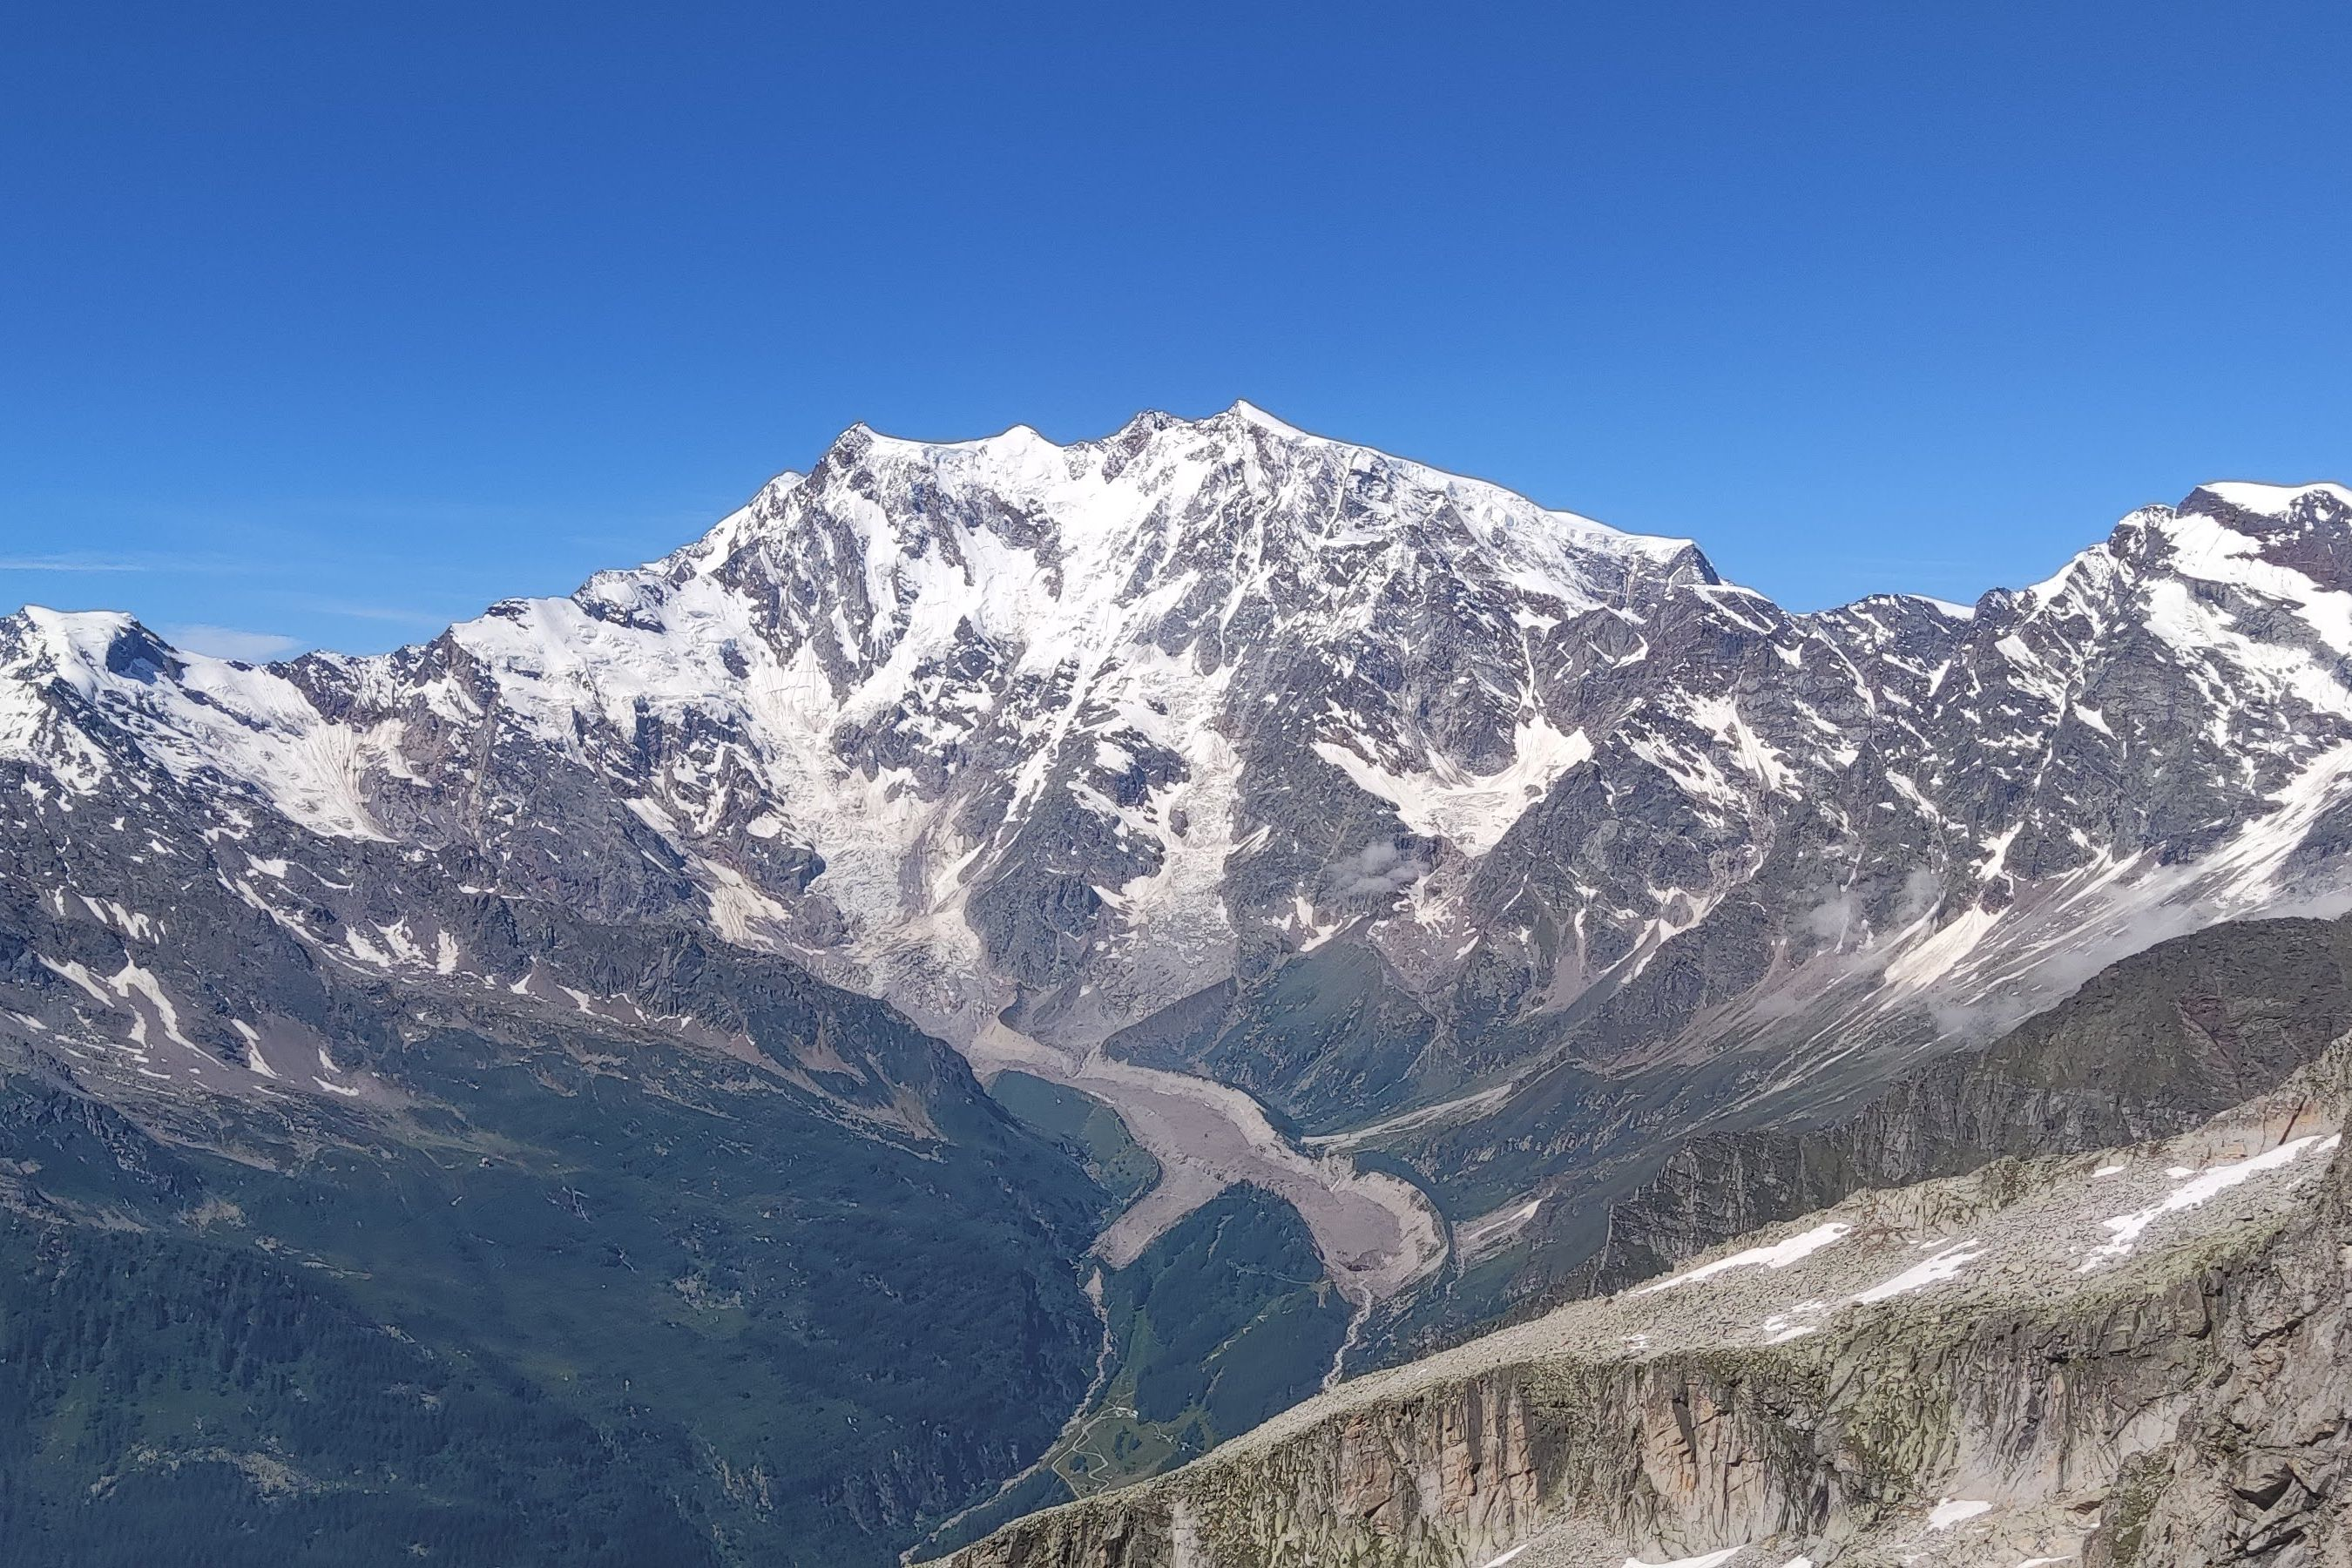
\includegraphics[height=5cm]{belvedere_pic.jpg}
    }
    \caption{(a) Location of Belvedere Glacier, base map (source: Swisstopo
        www.geo.admin.ch); (b) Picture of ...}
    \label{fig:1:studyarea}
\end{figure}

In the past, several hazardous events originated by the Belvedere Glacier, such as floods
and slope instability, threatened the nearby village of Macugnaga and the Zamboni Zappa
Hut,
at 2070 m a.s.l. \citep{Kaab2004}.
At the beginning of the 21st century, the Belvedere Glacier was characterized by a
particular
surge-type dynamics  \citep{Haeberli2002}.
During the late 1990s, the~surface speeds of the whole glacier were ranging between
\SIlist{30;45}{\meter\per\year}~\citep{Roethlisberger1985, Kaab2005}.
During 2000--2001 an accelerated flow in the Monte-Rosa Glacier produced a wave of
compression-decompression stresses and strains in the Belvedere Glacier.
Surface velocities soared: values up to \SI{200}{\meter\per\year} were observed
photogrammetrically during autumn 2001~\citep{Kaab2004}.
The ice thickness increased more than~\SI{20}{\meter} and the wave travelled downwards,
creating a depression area in the accumulation zone, that was filled by a super-glacial
lake, the~Lago Effimero~\citep{Haeberli2002, Mortara2009}.

% The northern lobe of the Belvedere Glacier is concurrently experiencing a fast retreat:
% in the past few years, an average retreat of \SI{\sim20}{\meter\per\year} was documented
% \citep{Ioli2022} and it is actively changing every day, due to ice falls and collapses.

% References
\makechapterbibliography{}